%%%% acra.tex

\typeout{ACRA Instructions for Authors}

% This is the instructions for authors for ACRA.
\documentclass{article}
\usepackage{acra}
\usepackage{lmodern}% http://ctan.org/pkg/lm
\usepackage{amsmath}
\usepackage{graphicx}
\usepackage{color}
\usepackage{hyperref}
\usepackage{amssymb}
\usepackage{url}
\usepackage{pdfpages}
\usepackage{fancyhdr}
\usepackage{subfig}
\usepackage{listings} 
\usepackage{selinput}    
\newcommand{\quotes}[1]{``#1''}

% The file acra.sty is the style file for ACRA. 
% The file named.sty contains macros for named citations as produced 
% by named.bst.

% The preparation of these files was supported by Schlumberger Palo Alto
% Research, AT\&T Bell Laboratories, and Morgan Kaufmann Publishers.
% Shirley Jowell, of Morgan Kaufmann Publishers, and Peter F.
% Patel-Schneider, of AT\&T Bell Laboratories collaborated on their
% preparation. 

% These instructions can be modified and used in other conferences as long
% as credit to the authors and supporting agencies is retained, this notice
% is not changed, and further modification or reuse is not restricted.
% Neither Shirley Jowell nor Peter F. Patel-Schneider can be listed as
% contacts for providing assistance without their prior permission.

% To use for other conferences, change references to files and the
% conference appropriate and use other authors, contacts, publishers, and
% organizations.
% Also change the deadline and address for returning papers and the length and
% page charge instructions.
% Put where the files are available in the appropriate places.

\title{Gaussian Process}
\author{Diego Garrido}

\begin{document}

\maketitle
\href{https://nbviewer.jupyter.org/github/dgarridoa/gaussian_process/blob/master/Gaussian_Process.ipynb}{\color{blue}{Jupyter Notebook}}

\section{Introduction}
A Gaussian Process (GP) define a prior over functions $f$, which can be converted into a posterior over functions once we have seen some data. Let $x_{1}, \ldots, x_{N}$ a set of point, a GP assumes that $p(f(x_{1}, \ldots, f(x_{N})))$ is jointly Gaussian, with some mean $\mu(x)$ and covariance $\Sigma(x)$ given by $\Sigma_{ij}=\kappa(x_{i}, x_{j})$, where $\kappa$ is a kernel function. In this work we sample from a multivariate gaussian (MVN) with different kernels, using this general setting: $N$=100, $x_{1}, \ldots, x_{N} = 0, \ldots, 99$ and $\mu(x)=0$.

\section{Square Exponential Kernel}

The squared exponential kernel is the more common kernel used. In Figure 1 we observe that to lower length scale ($\ell$) the function look more \quotes{wiggle}.

\begin{figure}[h]
\centering
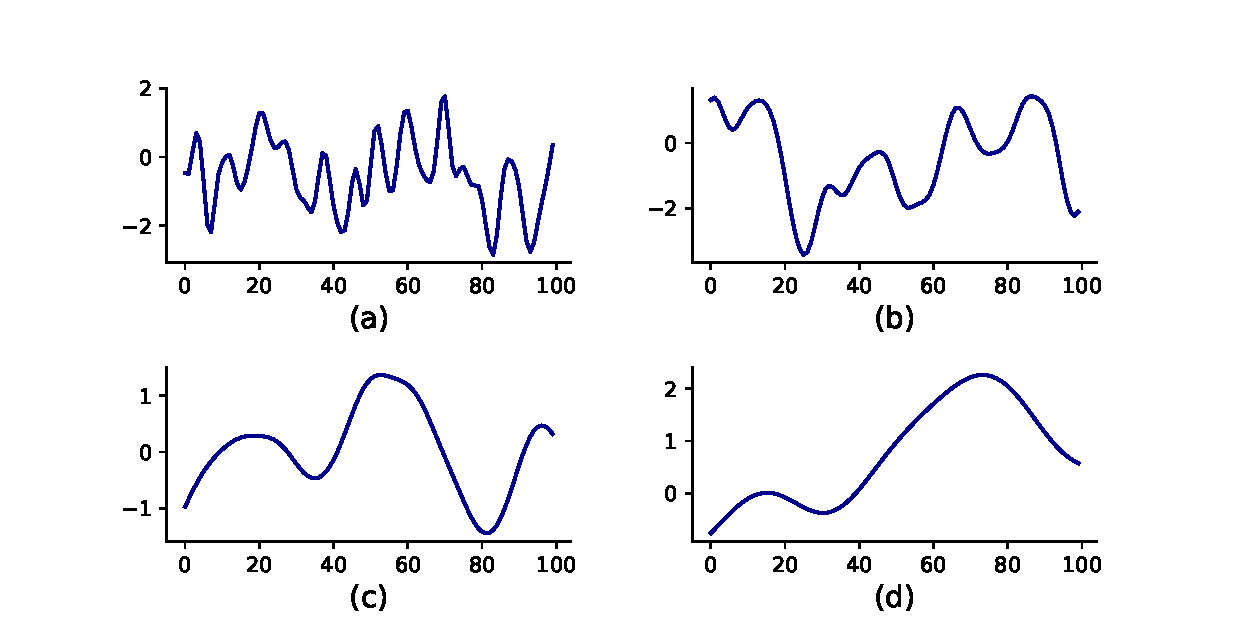
\includegraphics[scale=0.45]{img/square_exponential.eps}  
\caption{Samples from a MVN with square exponential kernel with $\mu=0$ and $\sigma=1$ for differents length scale ($\ell$). Axis x represent the support and axis y its values. (a) Plot with $\ell=1$, (b) $\ell=4$, (c) $\ell=8$ and (d) $\ell=16$.}
\end{figure}

\section{Locally Periodic Kernel}

This kernel is the product between the periodic kernel and the square exponential kernel. In Figure 2 we observe that to higher periodicity (p) lower is the distance between repetitions. Also, to difference of periodic kernel, this kernel allows periodicity without repeating exactly the same pattern, allowing variations over time that are smother to higher $\ell$.

\begin{figure}[h]
\centering
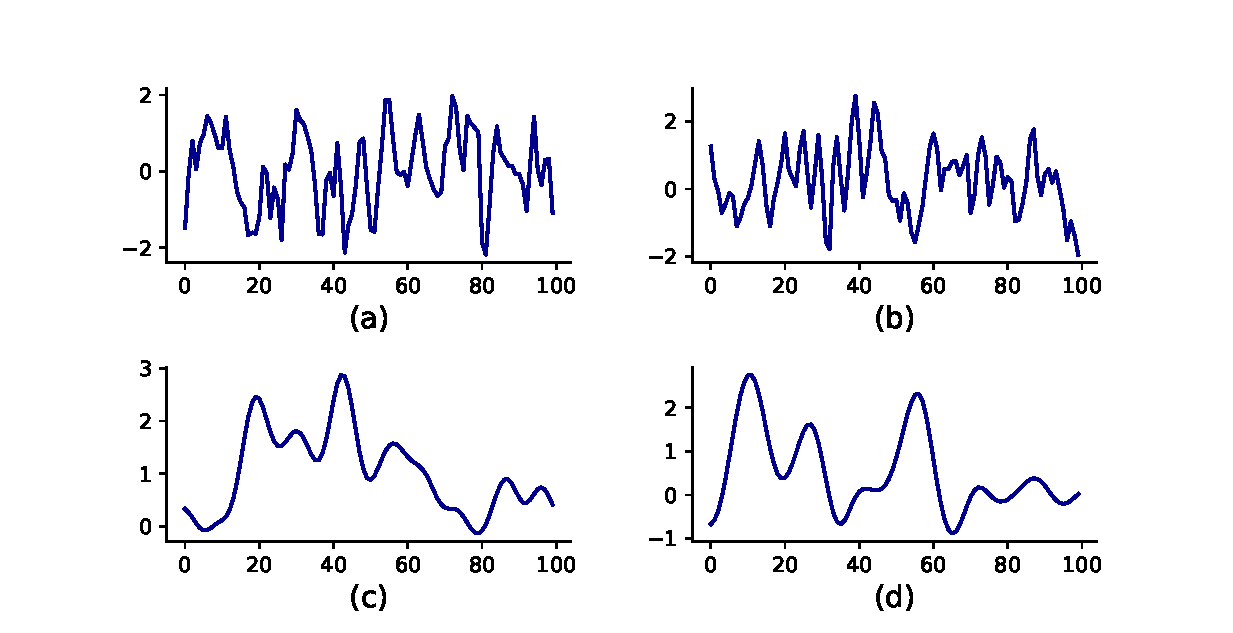
\includegraphics[scale=0.45]{img/locally_periodic.eps}  
\caption{Samples from a MVN with locally periodic kernel with $\mu=0$ and $\sigma=1$ for differents length scale ($\ell$) and periodicity ($p$). Axis x represent the support and axis y its values. (a) Plot with $(\ell=1, p=0.1 )$, (b) $(\ell=1, p=1)$, (c) $(\ell=5, p=0.1)$ and (d) $(\ell=5, p=1)$.}
\end{figure}



\section{Linear Plus Periodic Kernel}
This kernel is the sum between periodic kernel and linear kernel. In Figure 3 we have some samples from this kernel, we observe that this kernel result in a periodic function with increasing mean. The parameter $\sigma_{v}$ control the mean increment, that is higher to higher $\sigma_{v}$, on the other hand, the $\sigma_{b}$ parameter has an offset behavior, it determine how far from 0 the height of the function will be at zero.

\begin{figure}[h]
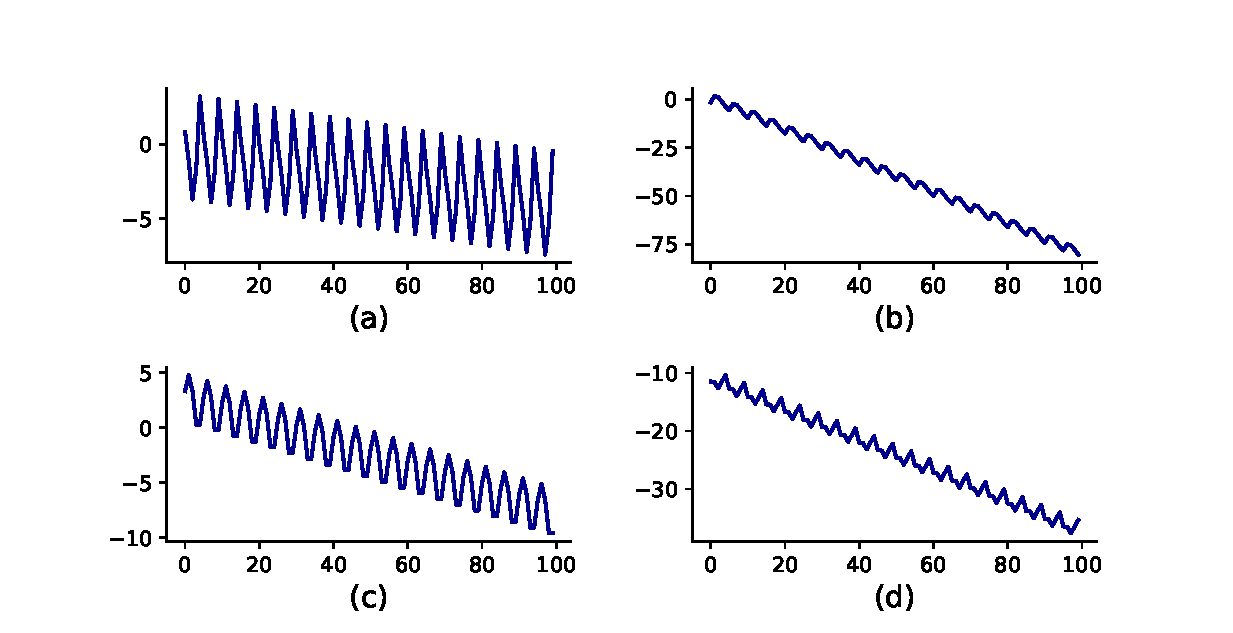
\includegraphics[scale=0.45]{img/linear_periodic.eps}  
\caption{Samples from a MVN with linear plus periodic kernel with $(\mu=0, \sigma=2, c=0, \ell=1, p=5)$ for differents $\sigma_{b}$ and $\sigma_{v}$. Axis x represent the support and axis y its values. (a) Plot with $(\sigma_{b}=0, \sigma_{v}=0.01)$, (b) $(\sigma_{b}=0, \sigma_{v}=0.1)$, (c) $(\sigma_{b}=4, \sigma_{v}=0.01)$ and (d) $(\sigma_{b}=4, \sigma_{v}=0.1)$.}
\end{figure}

\end{document}